\documentclass{standalone}
\usepackage{tikz}
\usetikzlibrary{patterns, positioning}


\begin{document}
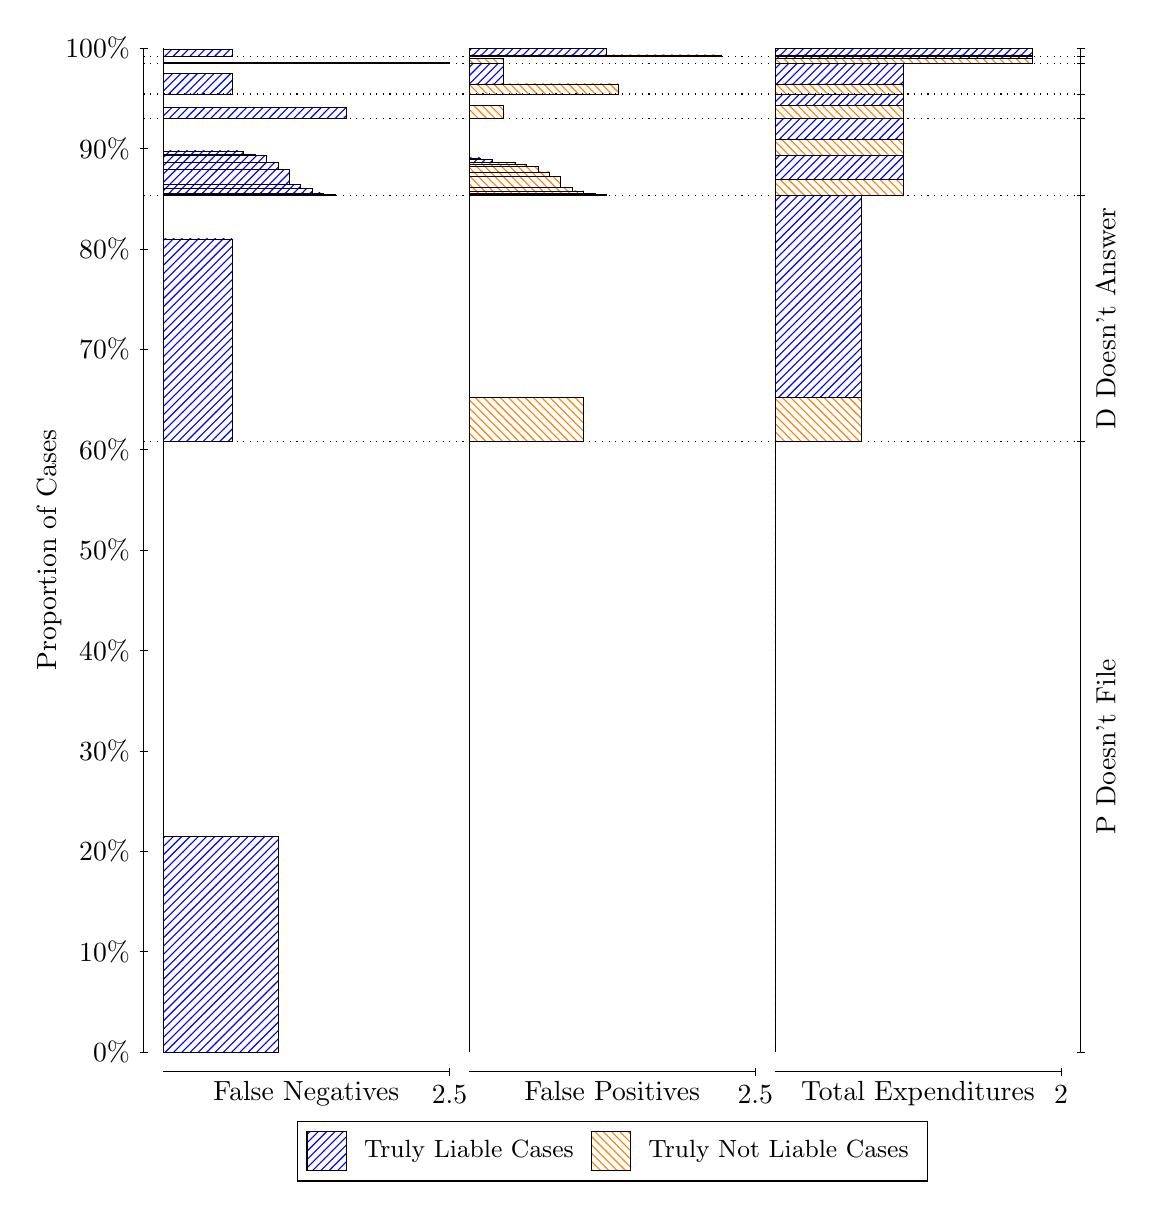
\begin{tikzpicture}
\draw[black, very thin] (1.5,1.75) -- (1.5,14.5);
\node[rotate=90, text=black, anchor=center] at (0.3, 8.125) {Proportion of Cases};
\draw[black, very thin] (1.45,1.75) -- (1.55,1.75);
\node[text=black, anchor=east] at (1.45, 1.75) {0\%};
\draw[black, very thin] (1.45,3.025) -- (1.55,3.025);
\node[text=black, anchor=east] at (1.45, 3.025) {10\%};
\draw[black, very thin] (1.45,4.3) -- (1.55,4.3);
\node[text=black, anchor=east] at (1.45, 4.3) {20\%};
\draw[black, very thin] (1.45,5.575) -- (1.55,5.575);
\node[text=black, anchor=east] at (1.45, 5.575) {30\%};
\draw[black, very thin] (1.45,6.85) -- (1.55,6.85);
\node[text=black, anchor=east] at (1.45, 6.85) {40\%};
\draw[black, very thin] (1.45,8.125) -- (1.55,8.125);
\node[text=black, anchor=east] at (1.45, 8.125) {50\%};
\draw[black, very thin] (1.45,9.4) -- (1.55,9.4);
\node[text=black, anchor=east] at (1.45, 9.4) {60\%};
\draw[black, very thin] (1.45,10.675) -- (1.55,10.675);
\node[text=black, anchor=east] at (1.45, 10.675) {70\%};
\draw[black, very thin] (1.45,11.95) -- (1.55,11.95);
\node[text=black, anchor=east] at (1.45, 11.95) {80\%};
\draw[black, very thin] (1.45,13.225) -- (1.55,13.225);
\node[text=black, anchor=east] at (1.45, 13.225) {90\%};
\draw[black, very thin] (1.45,14.5) -- (1.55,14.5);
\node[text=black, anchor=east] at (1.45, 14.5) {100\%};

\draw[black, very thin] (13.4,1.75) -- (13.4,14.5);
\draw[black, very thin] (13.35,1.75) -- (13.45,1.75);
\node[anchor=west] at (13.35, 1.75) {};
\draw[black, very thin] (13.35,9.5054) -- (13.45,9.5054);
\node[anchor=west] at (13.35, 9.5054) {};
\draw[black, very thin] (13.35,12.631) -- (13.45,12.631);
\node[anchor=west] at (13.35, 12.631) {};
\draw[black, very thin] (13.35,13.607) -- (13.45,13.607);
\node[anchor=west] at (13.35, 13.607) {};
\draw[black, very thin] (13.35,13.916) -- (13.45,13.916);
\node[anchor=west] at (13.35, 13.916) {};
\draw[black, very thin] (13.35,14.301) -- (13.45,14.301);
\node[anchor=west] at (13.35, 14.301) {};
\draw[black, very thin] (13.35,14.391) -- (13.45,14.391);
\node[anchor=west] at (13.35, 14.391) {};
\draw[black, very thin] (13.35,14.5) -- (13.45,14.5);
\node[anchor=west] at (13.35, 14.5) {};

\draw[black, very thin, pattern color=blue, pattern=north east lines] (1.75,1.75) rectangle (3.2033,4.4864);
\draw[black, very thin, pattern color=orange, pattern=north west lines] (1.75,4.4864) rectangle (1.75,9.5054);
\draw[black, very thin, pattern color=blue, pattern=north east lines] (1.75,9.5054) rectangle (2.622,12.077);
\draw[black, very thin, pattern color=orange, pattern=north west lines] (1.75,12.077) rectangle (1.75,12.631);
\draw[black, very thin, pattern color=blue, pattern=north east lines] (1.75,12.631) rectangle (3.93,12.645);
\draw[black, very thin, pattern color=blue, pattern=north east lines] (1.75,12.645) rectangle (3.7847,12.661);
\draw[black, very thin, pattern color=blue, pattern=north east lines] (1.75,12.661) rectangle (3.6393,12.714);
\draw[black, very thin, pattern color=blue, pattern=north east lines] (1.75,12.714) rectangle (3.494,12.773);
\draw[black, very thin, pattern color=blue, pattern=north east lines] (1.75,12.773) rectangle (3.3487,12.954);
\draw[black, very thin, pattern color=blue, pattern=north east lines] (1.75,12.954) rectangle (3.2033,13.049);
\draw[black, very thin, pattern color=blue, pattern=north east lines] (1.75,13.049) rectangle (3.058,13.133);
\draw[black, very thin, pattern color=blue, pattern=north east lines] (1.75,13.133) rectangle (2.9127,13.154);
\draw[black, very thin, pattern color=blue, pattern=north east lines] (1.75,13.154) rectangle (2.7673,13.193);
\draw[black, very thin, pattern color=orange, pattern=north west lines] (1.75,13.193) rectangle (1.75,13.607);
\draw[black, very thin, pattern color=blue, pattern=north east lines] (1.75,13.607) rectangle (4.0753,13.747);
\draw[black, very thin, pattern color=orange, pattern=north west lines] (1.75,13.747) rectangle (1.75,13.916);
\draw[black, very thin, pattern color=blue, pattern=north east lines] (1.75,13.916) rectangle (2.622,14.173);
\draw[black, very thin, pattern color=orange, pattern=north west lines] (1.75,14.173) rectangle (1.75,14.301);
\draw[black, very thin, pattern color=blue, pattern=north east lines] (1.75,14.301) rectangle (5.3833,14.322);
\draw[black, very thin, pattern color=orange, pattern=north west lines] (1.75,14.322) rectangle (1.75,14.391);
\draw[black, very thin, pattern color=blue, pattern=north east lines] (1.75,14.391) rectangle (2.622,14.479);
\draw[black, very thin, pattern color=orange, pattern=north west lines] (1.75,14.479) rectangle (1.75,14.5);
\draw[black, very thin, pattern color=orange, pattern=north west lines] (5.6333,1.75) rectangle (5.6333,6.7689);
\draw[black, very thin, pattern color=blue, pattern=north east lines] (5.6333,6.7689) rectangle (5.6333,9.5054);
\draw[black, very thin, pattern color=orange, pattern=north west lines] (5.6333,9.5054) rectangle (7.0867,10.059);
\draw[black, very thin, pattern color=blue, pattern=north east lines] (5.6333,10.059) rectangle (5.6333,12.631);
\draw[black, very thin, pattern color=orange, pattern=north west lines] (5.6333,12.631) rectangle (7.3773,12.643);
\draw[black, very thin, pattern color=orange, pattern=north west lines] (5.6333,12.643) rectangle (7.232,12.652);
\draw[black, very thin, pattern color=orange, pattern=north west lines] (5.6333,12.652) rectangle (7.0867,12.687);
\draw[black, very thin, pattern color=orange, pattern=north west lines] (5.6333,12.687) rectangle (6.9413,12.729);
\draw[black, very thin, pattern color=orange, pattern=north west lines] (5.6333,12.729) rectangle (6.796,12.866);
\draw[black, very thin, pattern color=orange, pattern=north west lines] (5.6333,12.866) rectangle (6.6507,12.927);
\draw[black, very thin, pattern color=orange, pattern=north west lines] (5.6333,12.927) rectangle (6.5053,12.999);
\draw[black, very thin, pattern color=orange, pattern=north west lines] (5.6333,12.999) rectangle (6.36,13.023);
\draw[black, very thin, pattern color=orange, pattern=north west lines] (5.6333,13.023) rectangle (6.2147,13.045);
\draw[black, very thin, pattern color=blue, pattern=north east lines] (5.6333,13.045) rectangle (5.924,13.084);
\draw[black, very thin, pattern color=blue, pattern=north east lines] (5.6333,13.084) rectangle (5.7787,13.105);
\draw[black, very thin, pattern color=blue, pattern=north east lines] (5.6333,13.105) rectangle (5.6333,13.607);
\draw[black, very thin, pattern color=orange, pattern=north west lines] (5.6333,13.607) rectangle (6.0693,13.776);
\draw[black, very thin, pattern color=blue, pattern=north east lines] (5.6333,13.776) rectangle (5.6333,13.916);
\draw[black, very thin, pattern color=orange, pattern=north west lines] (5.6333,13.916) rectangle (7.5227,14.044);
\draw[black, very thin, pattern color=blue, pattern=north east lines] (5.6333,14.044) rectangle (6.0693,14.301);
\draw[black, very thin, pattern color=orange, pattern=north west lines] (5.6333,14.301) rectangle (6.0693,14.371);
\draw[black, very thin, pattern color=blue, pattern=north east lines] (5.6333,14.371) rectangle (5.6333,14.391);
\draw[black, very thin, pattern color=orange, pattern=north west lines] (5.6333,14.391) rectangle (8.8307,14.412);
\draw[black, very thin, pattern color=blue, pattern=north east lines] (5.6333,14.412) rectangle (7.3773,14.5);
\draw[black, very thin, pattern color=orange, pattern=north west lines] (9.5167,1.75) rectangle (9.5167,6.7689);
\draw[black, very thin, pattern color=blue, pattern=north east lines] (9.5167,6.7689) rectangle (9.5167,9.5054);
\draw[black, very thin, pattern color=orange, pattern=north west lines] (9.5167,9.5054) rectangle (10.607,10.059);
\draw[black, very thin, pattern color=blue, pattern=north east lines] (9.5167,10.059) rectangle (10.607,12.631);
\draw[black, very thin, pattern color=orange, pattern=north west lines] (9.5167,12.631) rectangle (11.152,12.835);
\draw[black, very thin, pattern color=blue, pattern=north east lines] (9.5167,12.835) rectangle (11.152,13.134);
\draw[black, very thin, pattern color=orange, pattern=north west lines] (9.5167,13.134) rectangle (11.152,13.345);
\draw[black, very thin, pattern color=blue, pattern=north east lines] (9.5167,13.345) rectangle (11.152,13.607);
\draw[black, very thin, pattern color=orange, pattern=north west lines] (9.5167,13.607) rectangle (11.152,13.776);
\draw[black, very thin, pattern color=blue, pattern=north east lines] (9.5167,13.776) rectangle (11.152,13.916);
\draw[black, very thin, pattern color=orange, pattern=north west lines] (9.5167,13.916) rectangle (11.152,14.044);
\draw[black, very thin, pattern color=blue, pattern=north east lines] (9.5167,14.044) rectangle (11.152,14.301);
\draw[black, very thin, pattern color=orange, pattern=north west lines] (9.5167,14.301) rectangle (12.787,14.371);
\draw[black, very thin, pattern color=blue, pattern=north east lines] (9.5167,14.371) rectangle (12.787,14.391);
\draw[black, very thin, pattern color=orange, pattern=north west lines] (9.5167,14.391) rectangle (12.787,14.412);
\draw[black, very thin, pattern color=blue, pattern=north east lines] (9.5167,14.412) rectangle (12.787,14.5);
\draw[black, dotted] (1.5,9.5054) -- (13.4,9.5054);
\draw[black, dotted] (1.5,12.631) -- (13.4,12.631);
\draw[black, dotted] (1.5,13.607) -- (13.4,13.607);
\draw[black, dotted] (1.5,13.916) -- (13.4,13.916);
\draw[black, dotted] (1.5,14.301) -- (13.4,14.301);
\draw[black, dotted] (1.5,14.391) -- (13.4,14.391);
\draw[black, very thin] (1.75,1.5) -- (5.3833,1.5);
\node[text=black, anchor=north] at (3.5667, 1.5) {False Negatives};
\draw[black, very thin] (5.3833,1.45) -- (5.3833,1.55);
\node[text=black, anchor=north] at (5.3833, 1.45) {2.5};

\draw[black, very thin] (5.6333,1.5) -- (9.2667,1.5);
\node[text=black, anchor=north] at (7.45, 1.5) {False Positives};
\draw[black, very thin] (9.2667,1.45) -- (9.2667,1.55);
\node[text=black, anchor=north] at (9.2667, 1.45) {2.5};

\draw[black, very thin] (9.5167,1.5) -- (13.15,1.5);
\node[text=black, anchor=north] at (11.333, 1.5) {Total Expenditures};
\draw[black, very thin] (13.15,1.45) -- (13.15,1.55);
\node[text=black, anchor=north] at (13.15, 1.45) {2};

\node[text=black, centered, rotate=90] at (13.72, 5.6277) {P Doesn't File};
\node[text=black, centered, rotate=90] at (13.72, 11.068) {D Doesn't Answer};






\draw (7.449999999999999,1.5) node[draw=none] (baseCoordinate) {};
\begin{scope}[align=center]
        \matrix[scale=0.5, draw=black, below=0.5cm of baseCoordinate, nodes={draw}, column sep=0.1cm]{
            \node[rectangle, draw, minimum width=0.5cm, minimum height=0.5cm, pattern color=blue, pattern=north east lines] {}; &
            \node[draw=none, font=\small, text=black] (B) {Truly Liable Cases}; &
            \node[rectangle, draw, minimum width=0.5cm, minimum height=0.5cm, pattern color=orange, pattern=north west lines] {}; &
            \node[draw=none, font=\small, text=black] (B) {Truly Not Liable Cases}; \\
            };
\end{scope}

\end{tikzpicture}
\end{document}